\clearpage
\section{Begriffsabgrenzung \& Entwicklungen}\label{hauptabschnitt_2}
Da der E-Commerce immer wichtiger wird, ist es für Händler nicht mehr ausreichend, ihre Produkte und Dienstleistungen ausschließlich im stationären Handel anzubieten. Daher wird vom Autor empfohlen, sich regelmäßig mit den neuen Entwicklungen auseinanderzusetzen\footnote{Vgl. \autocite [Online] {Handelsverband2022}}.
So können die Wünsche der Kunden und Kundinnen langfristig erfüllt werden und die Wettbewerbsfähigkeit gegenüber der Konkurrenz stabil bleiben. Auf die Einstiegsmöglichkeiten in den Online-Handel wird im weiteren Verlauf der Arbeit genauer eingegangen.

\subsection{E-Commerce}\label{unterabschnitt_2_1}
\ac{eco} ist eine Abkürzung (zu deutsch: Elektronischer Handel) für den Begriff “Electronic Commerce” und umfasst den Online-Handel, der elektronisch, also im Internet stattfindet. Der Begriff umfasst alle Transaktionen des Handels (Kauf und Verkauf von Waren und Dienstleistungen jeglicher Art), die auf dem elektronischen Weg vollzogen werden\footnote{Vgl. \autocite [S. 19] {Deges2020}}.
Der E-Commerce beinhaltet verschiedene Handelsarten. Wenn ein privater Endkunde in einem Onlineshop einkauft, ist dies eine Business-to-Customer Logik, die oft mit \ac{b2c} abgekürzt wird. Zwischen zwei Unternehmen wird diese Beziehung Business-to-Business oder auch \ac{b2b} bezeichnet\footnote{Vgl. \autocite [S.50] {Heinemann2021}}.
\newline
Der Vertriebsweg sowohl für das B2B- als auch das B2C-Geschäft lässt sich auf zwei verschiedene Arten realisieren. Online-Shops stellen die Art des Direktvertriebs dar. Ein Unternehmen verkauft beispielsweise seine Artikel über einen eigenen Online-Shop.
\newline

Ein weiterer Vertriebsweg ist der Online-Marktplatz. Ein Online-Marktplatz ist eine Webseite, die als Verkaufsplattform dient und auf der sich unterschiedliche Käufer und Verkäufer elektronisch begegnen.
\newline

Als die erfolgreichsten Vertreter:innen dieser Vertriebsart galt lange Zeit das amerikanische Unternehmen eBay, das 1995 gegründet wurde. Vor einigen Jahren wurde eBay von Amazon Marketplace als der erfolgreichste Online-Marktplatz abgelöst\footnote{Vgl. \autocite [Online] {Feldkircher2020}}.
\newline

Durch den Online-Marktplatz-Gigant Amazon entwickelte sich das (\ac{fba}) zu einem beliebten Serviceangebot. Beim FBA zahlt der Verkäufer eine Gebühr an Amazon für Dienstleistungen eines oder mehrerer Produkte. Amazon bietet dann die Produkte auf seinem Portal an und übernimmt sowohl die Produktlagerung als auch den Versand an den Käufer. Für den Verkäufer hat dieses die Vorteile, dass keine Lagerung mehr nötig ist, der Versand erfolgt innerhalb kürzester Zeit ohne jeglichen Aufwand und Amazon bietet die Lieferung an Premiumkunden und Premiumkundinnen versandkostenfrei an.

\subsubsection{Abgrenzung des E-Commerce zum E-Business}\label{unterabschnitt_2_1_1}
Oftmals werden die Begriffe E-Commerce und \ac{ebu} als Synonyme füreinander verwendet. Der E-Commerce beschreibt jedoch nur einen Teil des E-Business und bezieht sich auf den Kauf und Verkauf von Waren und Dienstleistungen über das Internet. E-Commerce ist ein Teilbereich des E-Business, der sich auf die Transaktionen zwischen Unternehmen und Kunden oder Kundinnen konzentriert. E-Commerce umfasst sowohl Business-to-Consumer (B2C), bei dem Unternehmen direkt an Endverbraucher verkaufen, als auch Business-to-Business (B2B), bei dem Unternehmen gegenüber anderen Unternehmen verkaufen.
\newline

Das E-Business umfasst dabei noch weitere Prozesse, die ein Unternehmen über das Internet in Anspruch nehmen kann\footnote{ Vgl. \autocite [S.71] {Meidl2014}}.
\newline
Der Begriff E-Business bezieht sich auf die Verwendung von elektronischen Technologien, um alle Geschäftsprozesse zu optimieren und zu automatisieren. Dies umfasst alle Aktivitäten, die für den Betrieb eines Unternehmens erforderlich sind, wie beispielsweise die interne Kommunikation, die Kundenbetreuung, die Buchhaltung und die Personalverwaltung.


\subsubsection{Entwicklung des E-Commerce}\label{unterabschnitt_2_1_2}
Im Jahr 2021 wurden, wie in den Jahren zuvor, erneut neue Rekordzahlen geschrieben. Es wurden im Bereich E-Commerce durch Online-Einkäufe alleine in Deutschland ca. 87 Milliarden Euro umgesetzt.
\newline
Auch wenn die beiden Pandemie Jahre 2020 und 2021\footnote{Vgl. \autocite [Online] {Wikipedia2019}} nahezu alle Prognosen weit übertroffen haben, gab es im Jahr 2021 verglichen mit dem Vorjahr nochmal einen Anstieg des Umsatzes um mehr als 19\%, was das Potenzial des E-Commerce für die Zukunft nochmal verdeutlicht. Seit 2006 konnte der E-Commerce in Deutschland kontinuierlich steigenden Umsatz verzeichnen. Bei der Auswertung stellt sich heraus, dass die Marktplätze ihre Marktposition weiter ausbauen und vor allem stationäre Händler diese Option nutzen, um im Onlinehandel präsent zu sein.
\newline

Im Geschäftsjahr 2021 wurden von den Käufern über 50\% aller Online Einkäufe über das Smartphone getätigt. Es zeigt sich eine klare Tendenz, dass Verbraucher immer mobiler werden. Für die nächsten Jahre wird prognostiziert, dass der Umsatz kontinuierlich ansteigen wird\footnote{Vgl. \autocite [Online] {Handelsverband2022}}.

\begin{figure}[!ht]
    \centering
    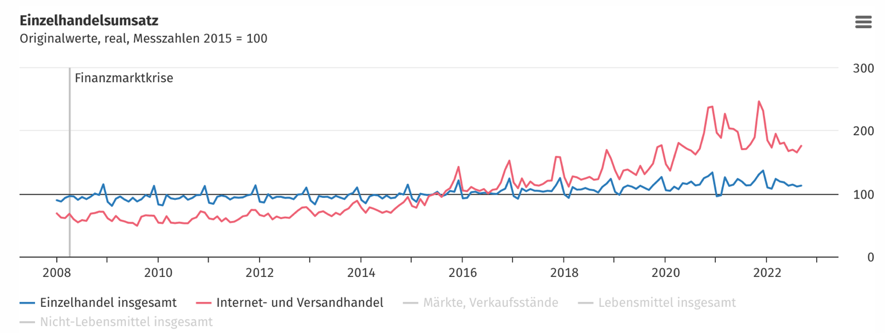
\includegraphics[width=1\textwidth,angle=0]{src/abbildungen/onlineVsEinzelhandel.png}
    \caption[Quelle: Statistisches Bundesamt, 2022]{Umsatzentwicklung von 2008 bis 2022 - Einzelhandel vs. Versandhandel, Quelle: \autocite {Bundesamt2022}}
   \label{fig: Statistisches_Bundesamt}
   \end{figure}

Die vorliegende Grafik visualisiert, dass der Internet- und Versandhandel gegenüber dem Einzelhandel seit 2014 kontinuierlich Konsumierende für sich gewann. Wie die Grafik zudem aufzeigt, übertraf im Jahr 2015 der Umsatz des Internethandels erstmals den des stationären Einzelhandels. Es lässt sich zudem erkennen, dass der Umsatz des Einzelhandels nicht fällt. Allerdings muss auch beachtet werden, dass der Markt stetig wächst und das Wachstum im Einzelhandel hingegen stagniert.


\subsection{Stationärer Einzelhandel}\label{unterabschnitt_2_3}
„Stationärer Handel ist der Sammelbegriff für Handelsbetriebe mit festem Standort“\footnote{Vgl. \autocite [S.23] {Heinemann2011}}.
\newline
Der stationäre Handel ist ein fester Standort, an dem Produkte oder Dienstleistungen zum Kauf angeboten werden. Traditionell wird das Produkt bei einem Kauf direkt mitgenommen.
\newline

Im Optimalfall erleben die Besucher:innen ein Einkaufserlebnis, indem Produkte vor Ort angesehen, taktil wahrgenommen oder auch gerochen werden können. Zudem können sich die Besucher:innen von dem Verkaufspersonal zu den Produkten beraten lassen. Das Kaufverhalten der Besucher:innen wird beeinflusst und der Kaufimpuls gesteigert\footnote{ Vgl. \autocite [S.71] {Buttkus2019}}.
\newline

Ursprungsgemäß sind die Zielgruppe eines stationären Handels Besucher:innen, die zunächst ohne Bedürfnisse den Handel betreten. Während des Besuches wechselt diese Absicht jedoch und es wird für interessant erscheinende Produkte das Kaufempfinden erweckt\footnote{Vgl. \autocite [S.53] {Heinemann2021}}.


\subsubsection{Entwicklung des stationären Einzelhandels}\label{unterabschnitt_2_3_1}
In den letzten Jahrzehnten haben sich die Anforderungen des stationären Einzelhandels verändert. Die ersten Handelsformen waren kleine Einzelhandelsgeschäfte, die Lebensmittel und andere Artikel des täglichen Bedarfs anboten. Die Artikel waren auf die Funktionalität ausgerichtet. Durch die stetige Nachfrage gibt es heute große und moderne Einkaufszentren für verschiedene Branchen\footnote{Vgl. \autocite [S.3] {Jaeger2016}}.
\newline

Wie Abbildung 1 zeigt, entscheiden sich mittlerweile in vielen Branchen immer mehr Verbraucher häufiger für den Online-Einkauf. Einzelhandelsunternehmen erleiden zum Teil negative Nebenwirkungen, wenn Käufer:innen nicht mehr vor Ort ein, sondern sich für den für sie bequemeren Weg entscheiden, online einzukaufen\footnote{Vgl. \autocite [S.11] {Deichner2022}}.
\newline

Auswertungen zufolge bevorzugte im Jahr 2021 etwas weniger als jeder zweite Konsumierende (46 Prozent) den stationären Handel. Daraus lässt sich schließen, dass der Einzelhandel noch immer von hoher Bedeutung ist\footnote{Vgl. \autocite [Online] {Bundesamt2022}}. Auch die gleichbleibenden Umsätze zeigen deutlich auf, dass der stationäre Einzelhandel noch immer von wichtiger Bedeutung ist.
\newline

Der Einzelhandel kann bei vielen von Konsumierenden geforderten Punkten dem E-Commerce allerdings nicht standhalten. Durch den starken Wettbewerb im E-Commerce wird der Preis von großen Unternehmen gedrückt, wodurch viele kleine Unternehmen nicht wettbewerbsfähig agieren können und um ihre Existenz kämpfen müssen.
\newline

Für den Einzelhandel besteht die Herausforderung, dynamisch agieren und schnellstmöglich auf Veränderungen reagieren zu können. Die Corona-Pandemie beispielsweise traf viele kleinere Unternehmen, weil diese zum Teil über Monate aufgrund der Lockdowns ihre Geschäfte nicht öffnen durften. Online-Shops hingegen sind dauerhaft erreichbar und Pakete kommen in der Regel innerhalb weniger Werktage bei dem Kunden oder der Kundin an. An diese Flexibilität und Bequemlichkeit gewöhnen sich Konsumierende schnell, wenn ein gesuchtes Produkt über Suchmaschinen von vielen Online-Shops angeboten wird. Durch diese dauerhafte Erreichbarkeit und Verfügbarkeit eines Produkts werden neue Anforderungen an den Einzelhandel gestellt. Dadurch steigt der Anspruch der Kundschaft, der Einzelhandel allerdings wird diesem Anspruch nicht gerecht und klafft bei vielen Kunden mit der Zufriedenheit auseinander\footnote{Vgl. \autocite [S.3] {Jaeger2016}}.

\begin{figure}[!ht]
    \centering
    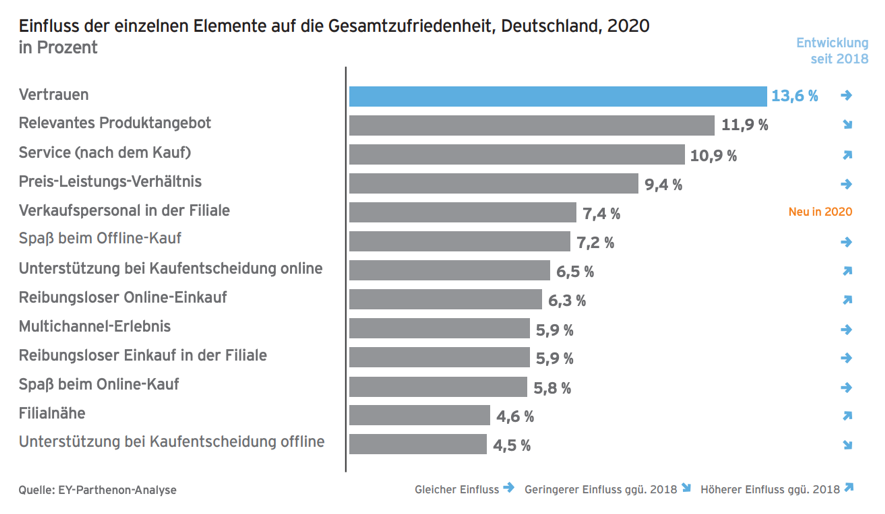
\includegraphics[width=1\textwidth,angle=0]{src/abbildungen/gesamtzufriedenheit_verbraucher.png}
    \caption[Quelle: EY-Parthenon-Analyse, 2020]{EY-Parthenon-Analyse, Quelle: \autocite {EYParthenon2020}}
   \label{fig: Quelle: EY-Parthenon-Analyse 2020}
   \end{figure}

Bei dieser repräsentativen Studie wurden Konsumierende in mehreren europäischen Ländern und in den USA nach ihrer Wahrnehmung des Leistungsversprechens befragt.
\newline
Es ist eine klare Tendenz erkennbar, dass aus Kundensicht beliebte Faktoren für die Kundenzufriedenheit wie Produktangebot oder Preis-Leistungs-Verhältnis von großen Unternehmen im Internet einfacher anzubieten sind, als von Einzelhandelsunternehmen.
Auch bei der Qualifikation des Verkaufspersonals oder einem ansprechenden Ambiente herrscht bei vielen Einzelhandelsunternehmen Nachholbedarf.
\newline

Unternehmen sollten zum Beispiel den Vorteil nutzen, mit guten Verkaufsberatungen vor Ort die Zufriedenheit des Kunden zu wecken und diesen in den Mittelpunkt zu stellen. Für den stationären Einzelhandel wäre es wichtig, mit Freundlichkeit und Expertise den Kunden zu überzeugen und beim Kaufen zu unterstützen.


\subsection{Der Begriff Kosmetik}\label{unterabschnitt_2_5}
Der Begriff Kosmetik bezieht sich auf Produkte und Dienstleistungen, die zur Verbesserung des Aussehens und der Schönheit von Haut, Haaren und Nägeln verwendet werden. Kosmetikprodukte umfassen in der Regel Hautpflegeprodukte, dekorative Kosmetik (Make-up), Parfüm, Haarpflegeprodukte und Produkte für die Nagelpflege.
\newline

Hautpflegeprodukte umfassen verschiedene Arten von Cremes, Lotionen, Serums und Masken, die dazu verwendet werden, die Haut zu pflegen, zu befeuchten und zu schützen. Sie können auf verschiedene Hauttypen und -bedürfnisse abgestimmt sein und bestehen aus verschiedenen Inhaltsstoffen, darunter Feuchthaltemittel, Fette und Öle, Vitamine und Pflanzenextrakte\footnote{Vgl. \autocite [S. 11] {Umbach2012}}.
\newline

Make-up umfasst verschiedene Arten von Produkten, die verwendet werden, um das Aussehen der Haut, der Augen, der Lippen und der Wangen zu verbessern. Dazu gehören beispielsweise Foundations, Concealer, Rouge, Lidschatten, Mascara und Lipgloss. Make-up kann in verschiedenen Formen erhältlich sein, darunter Flüssigkeiten, Cremes und Pulver.
Parfüm ist ein Duftstoff, der in einer Flüssigkeit oder einer Creme suspendiert ist und zur Verbesserung des Körpergeruchs verwendet wird. Es gibt viele verschiedene Arten von Parfüm, die auf verschiedene Weise hergestellt werden und unterschiedliche Duftnoten aufweisen.
\newline

Haarpflegeprodukte umfassen verschiedene Arten von Shampoo, Conditioner, Haaröl und anderen Produkten, die zur Pflege und Styling von Haaren verwendet werden. Sie können auf verschiedene Haartypen und -bedürfnisse abgestimmt sein und bestehen aus verschiedenen Inhaltsstoffen, darunter Feuchthaltemittel, Proteinen, Ölen und Pflanzenextrakten.
Produkte für die Nagelpflege umfassen verschiedene Arten von Lacken, Reinigern und anderen Produkten, die zur Pflege und Verschönerung von Nägeln verwendet werden. Dazu gehören beispielsweise Nagelfeile, Nagelknipser, Nagelpflegelacke und Nagelhärter.
\newline

Bei der Herstellung von Kosmetikprodukten müssen rechtliche Grundlagen erfüllt werden. In Europa unterliegen Kosmetikprodukte der \ac{eu}-Kosmetikverordnung, die Anforderungen an die Sicherheit, Kennzeichnung und Notifizierung von Produkten festlegt. In anderen Regionen der Welt gelten hingegen andere Regelungen. Es ist wichtig, sich über die geltenden Gesetze und Vorschriften in dem Land zu informieren, in dem das Produkt hergestellt und verkauft werden soll\footnote{Vgl. \autocite [online] {Haendlerbund2013}}.

\subsubsection{Entwicklung der Kosmetikbranche in Deutschland}\label{unterabschnitt_2_5_1}
Mit Blick auf die vergangenen 10 Geschäftsjahre ist das Marktvolumen von Kosmetik- und Körperpflegeprodukten, mit Ausnahme der Pandemiejahre 2020-2021, kontinuierlich angestiegen und bewegte sich 2013 bei 13,6 Milliarden Euro Umsatz und im Jahr 2021 bei knapp 16 Milliarden Euro Umsatz. Für das Jahr 2022 wurde im August 2022 ein Jahresumsatz von 15,75 Milliarden prognostiziert. Aufgrund der Ausbreitung des COVID-19-Virus folgte deutschlandweit die vorübergehende Schließung vieler stationärer Geschäfte. In dieser Zeit konnten viele Unternehmen zum Teil über Monate keinen Umsatz durch das Ladengeschäft generieren. In den Zahlen machte sich dies deutlich, indem der Umsatz im Einzelhandel in der Kosmetikbranche über diesen Zeitraum um 15 Prozent sank\footnote{Vgl. \autocite [Online] {statista2022}}.
\newline

Ein Großteil der Kosmetikprodukte kauften die Kunden während dieser Zeit über den Online-Handel.
\newline
Gezwungenermaßen waren Unternehmen dazu aufgefordert, die Sicht auf das Online-Geschäft zu erweitern, um die Kundenbedürfnisse zufrieden zu stellen und den Umsatz möglichst aufrechtzuerhalten.
\newline
Die Kosmetikbranche hat sich im Laufe der Pandemie den Herausforderungen gestellt und als widerstandsfähig erwiesen.
\newline

Durch die Revolution des Online-Geschäfts und vieler neuer Technologiemöglichkeiten wie dem sprachbasiertem Online-Einkauf über Sprachassistenten wie Alexa wurden in den vergangenen Jahren neue Einkaufsmöglichkeiten gesetzt, wodurch automatisch auch die Kundenanforderungen gestiegen sind und eine neue Erwartungshaltung entstanden ist.
\newline

Eine schlechte Onlinepräsenz nimmt den Unternehmen die Reichweite, um Kunden für sich zu gewinnen und Kundenbedürfnisse zu befriedigen.
\newline

Die Entwicklung zum branchenübergreifenden Online- und Versandhandel ist jedoch nicht erst seit Corona aktuell, sondern wie in Punkt 2.1.2. beschrieben, ein Prozess, der kontinuierlich verlief. Die Corona Pandemie war ein weiterer Indikator, wie wichtig es für Unternehmen ist, die neuen Technologien gewinnbringend zu nutzen und als Unternehmen zu wachsen.
\newline
Mittlerweile kann der E-Commerce als passende Ergänzung zum Online-Shop genutzt werden. Der E-Commerce dient nicht nur als gute Erweiterung, sondern bietet auch neue Möglichkeiten, sodass beide Handelsarten erfolgreich miteinander kombinieren können.
\newline

Auch in Bezug auf die Herstellung der Kosmetikprodukte veränderten sich durch die Sichtweise der Konsumierenden in den letzten 10 Geschäftsjahren die Anforderungen für die Herstellung der Kosmetikprodukte. Es wird vermehrt auf Produkte bestehend aus zwei Ansätzen gesetzt. Diese bestehen zum einen aus der Wirkstoffkosmetik und zum anderen aus der Naturstoffkosmetik. Produkte aus der Wirkstoffkosmetik sorgen nachweislich dafür, die Haut zu verbessern. Naturstoffkosmetik Produkte basieren auf rein pflanzlicher Herstellung. Der Trend der Konsumierenden verläuft eindeutig in die Richtung, vegane Produkte zu kaufen. Aus diesem Grund sind die Unternehmen dazu aufgefordert, Produkte aus der Naturstoffkosmetik anzubieten\footnote{Vgl. \autocite [Online] {Verbraucherzentrale2022}}.


\subsection{Grundlagen der verschiedenen Handelsarten}\label{hauptabschnitt_2_grundlagen}
Um sich dem Phänomen des Omni-Channel-Retailing (=Einzelhandel) zu nähern, ist es hilfreich, den Begriff zu definieren und abzugrenzen. Sowohl in den Medien als auch in der Praxis werden in diesem Zusammenhang oft die Begriffe Multi-Channel- und Cross-Channel-Handel genutzt. Es handelt sich hierbei zwar um ähnliche Handelsformate, allerdings bauen diese aufeinander auf und sind jeweils von ihrem Vorgänger abzugrenzen.

\newpage

\begin{figure}[!ht]
    \centering
    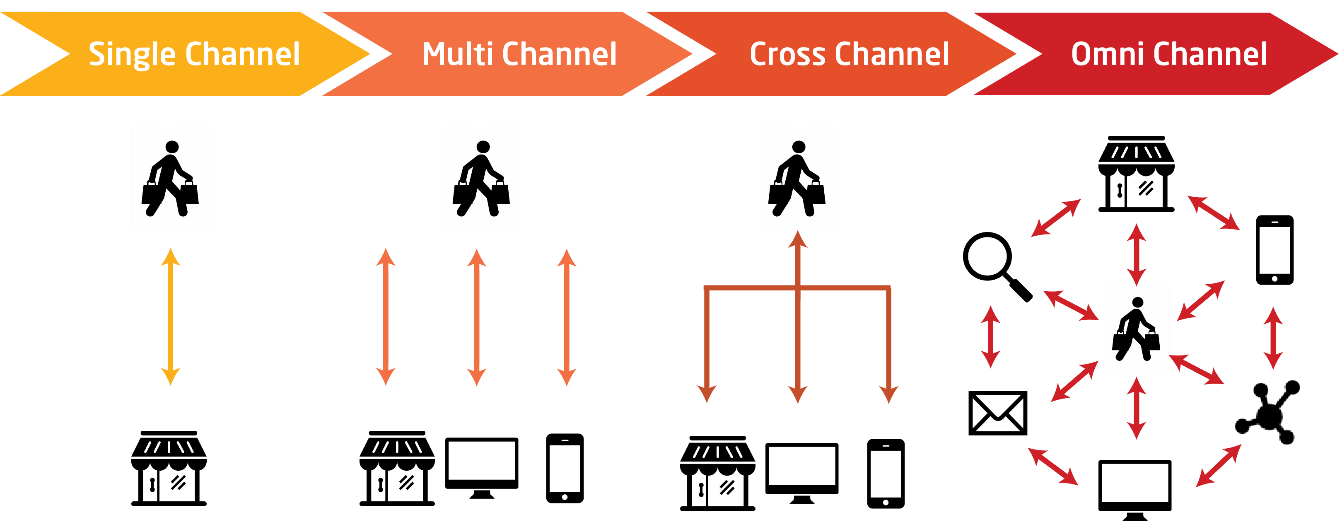
\includegraphics[width=0.95\textwidth,angle=0]{src/abbildungen/verkaufskanaele.png}
    \caption[Quelle: Multi-Channel, Omni-Channel oder Personalisierung, 2022]{Entwicklung der verschiedenen Geschäftsmodelle in Anlehnung an Talin , Quelle: \autocite {Talin2022}}
   \label{Onlineshopping_smartphone}
   \end{figure}
\newline

Im Folgenden wird Geschichtliches zu den Begriffen erläutert und wie diese Handelsformate entstanden sind. Zudem werden in diesem Zusammenhang benutzte Fachbegriffe erläutert.

\subsubsection{Single-Channel-Handel}\label{unterabschnitt_2_2_1}
Übersetzt bedeutet der Begriff Single-Channel „Einzel-Kanal“. Bezogen auf den Handel wird bei Single-Channel-Strategien von Händlern gesprochen, die einzig und allein über einen Vertriebskanal verfügen. Dies kann zum Beispiel der Online-Shop alleine oder ein stationärer Verkaufsladen sein. Erwähnenswert ist, dass die Online-Pure-Player, die „nur“ über einen Online-Marktplatz verfügen, ebenfalls zu der Kategorie des Single-Channel-Anbieters zählen. Weitere Beispiele sind zum Beispiel ein Schreibwarenladen, der lediglich innerhalb dessen Geschäfts die Waren verkauft.


\subsubsection{Multi-Channel-Handel}\label{unterabschnitt_2_2_2}
Multi-Channel-Retailing (Handel über mehrere Vertriebswege) zeichnet aus, dass ein Unternehmen Besucher:innen und potenzielle Kunden und Kundinnen über mehr als nur einen Verkaufskanal bzw. Vertriebsweg erreichen kann. So soll die Erreichbarkeit des Unternehmens an die Kundschaft erhöht und die Umsätze gesteigert werden\footnote{Vgl. \autocite [S.20] {Wirtz2022}}.
Ein Unternehmen bietet beim Einsatz einer Multi-Channel-Strategie verschiedene Vertriebskanäle an.
\newline

Ein Vertriebskanal oder Verkaufskanal lässt sich zunächst in zwei Kategorien unterteilen. Bei der Art des direkten Vertriebskanals verkauft ein Unternehmen seine Produkte direkt an die Konsumierenden bzw. Verbraucher:innen. Beispiele sind unter anderem der direkte Vertrieb vor Ort an den Endkunden oder über den eigenen Online-Shop. Bei indirekten Vertriebskanälen sind Zwischenhändler involviert, die dabei unterstützen sollen, einen größeren Kundenstamm für das Unternehmen zu erreichen. Beispiele sind Einzelhändler, Großhändler oder Online-Marktplätze wie Amazon\footnote{Vgl. \autocite [Online] {GisclardBiondi2021}}.
\newline

Der Begriff Multi-Channel-Retailing wurde vor knapp 140 Jahren zum ersten Mal in diesem Kontext genutzt, als die kanadische Warenhauskette Timothy Eaton den ersten Versandkatalog weltweit herausgebracht hat\footnote{Vgl. \autocite [Online] {Santink2015}}.
\newline

Der Versandhändler Otto hat 2021/2022 einen Jahresumsatz von über 16 Milliarden Euro verbucht und gehört heutzutage nicht nur zu den erfolgreichsten Onlinehändlern in Europa, sondern ist einer dieser Giganten, der die Stärken des Multichannel-Retailing bereits 1949 mit seinem ersten Versandkatalog erkannt und im Laufe der Zeit perfektioniert hat\footnote{Vgl. \autocite [Online] {Otto2022}, \autocite [Online] {Rabe2022}}.
\newline

Zudem kam neben dem Versandhandel seit 1995 der Onlinehandel hinzu, der sich durch die Digitalisierung, mit dem Beginn der Erfindung des Internets, weiter verändert hat. Bei vielen Unternehmen folgte im Laufe der Jahre ein Umdenken der Unternehmensstrategie, weil der Wettbewerb nicht mehr nur regional vertreten war, sondern sich global verlagerte. Dadurch, dass der Onlinehandel neue Maßstäbe setzen konnte, die von nun an die Bedürfnisse der Kunden deckten, entwickelte sich der Onlinehandel für den stationären Handel zu einer großen Konkurrenz.
\newline

Große Online Pure Player\footnote{Vgl. \autocite [Online] {Deges2020a}} wie Alibaba, Amazon oder eBay, die ihren Vertrieb ausschließlich über den Distanzhandel\footnote{Vgl. \autocite [Online] {Schneider2018}} betreiben, können ihren Kunden eine größere Produktauswahl zu besseren Konditionen anbieten. Eine rund um die Uhr Erreichbarkeit mit einem 24/7 Service (24 Stunden am Tag und 7 Tage pro Woche verfügbar) ist keine Seltenheit mehr. Von der Bestellung zur Versandabwicklung bis vor die Tür vergehen in der Regel nur wenige Tage.\footnote{Vgl. \autocite [S.17] {Vallee2018}}
\newline

Eine mögliche Umsetzungsart, weiterhin wettbewerbsfähig zu sein, ist für viele Einzelhandelsunternehmen die Einsetzung einer Multi-Channel-Strategie, indem sie zusätzlich zu ihrem stationären Handel einen Onlineshop aufbauen.


\subsubsection{Cross-Channel-Handel}\label{unterabschnitt_2_2_3}
Vor einem Jahrzehnt stellten sich viele Unternehmen noch die Frage, ob es notwendig sei, auch einen Onlineshop zu betreiben, um den Kundenstamm zu erweitern oder konkurrenzfähig zu bleiben. Heute stellen sich diese Unternehmen viel mehr die Frage, ob das Filialgeschäft mit dem Onlinekanal besser verknüpft werden muss. Beide Fragen sind klar mit ja zu beantworten, denn wenn ein Unternehmen es selbst nicht früh genug in die Hand nimmt, finden sich Konkurrenzunternehmen, die nicht zögern und Kundenbedürfnisse für die Zukunft besser befriedigen können.
\newline

2016 zeigte das \ac{ehi} Retail Institut mit einer Studie, wie fortgeschritten der Trend zum Onlinehandel bereits ist\footnote{Vgl. \autocite [S.17] {Hofacker2016}}.  Mehr als 70 Prozent der befragten Handelsunternehmen schätzten bereits 2016 das Click \& Collect Konzept, bei der die Ware online bestellt werden kann und in der nächstgelegenen Filiale abgeholt werden kann, als wichtig ein.
\newline

Über zwei Drittel der Befragten empfinden auch die Online-Bestandsabfrage als sehr sinnvoll ein, ebenso wie das Angebot eines Instore-Returns. Ein Instore-Return ist ein über den Onlineshop gelieferter Artikel, der vor Ort wieder returniert werden kann.
\newline

Bei der Cross-Channel-Integration spielt die Vernetzung der Online- und Offlinekanäle eine entscheidende Rolle.
\newline
Das Cross-Channel-Retailing erweitert das Multi-Channel-Verfahren und man spricht von Cross-Channel-Integration, sobald die ersten Verkaufskanäle miteinander verknüpft sind. Für Kunden entsteht dadurch die Möglichkeit, das Einkaufserlebnis kanalübergreifend zu gestalten, indem der Einkauf über verschiedene Verkaufskanäle abgewickelt werden kann. Darin enthalten sind zum Beispiel die Bestellung als Click \& Collect aufzugeben. Weitere Begriffe sind das \ac{fba} oder auch der \ac{b2b}-Handel
\newline

Mit der Verknüpfung der Verkaufskanäle gibt ein Unternehmen aber nicht nur den Kunden neue Möglichkeiten. Mitarbeiter können unter anderem Produkt- oder Kundendaten abfragen und dem Kunden so ein verbessertes Feedback über Produktfragen bieten.


\subsubsection{Omni-Channel-Handel}\label{unterabschnitt_2_2_4}
Der Begriff „omni“ stammt aus dem Lateinischen. Omni bedeutet so viel wie „alle“, „alles“, oder „ganz“\footnote{Vgl. \autocite [Online] {Wortbedeutung.info2022}}.
\newline
Wie bereits in Punkt 3 beschrieben, legt das Single-Channel-Marketing eine Basis für alle anderen Channel Arten, die aufeinander aufbauen. Um die Wichtigkeit zu verdeutlichen, ist Omni-Channel-Retailing zwar eine Weiterentwicklung des Multi-Channel-Verfahrens, doch diese ist grundlegend und damit ein wesentlicher Teil des Omni-Channel-Retailing.
\newline

Im Omni-Channel-Retailing werden die Daten der verschiedenen Kanäle miteinander verbunden und zentralisiert, sodass alle Plattformen perfekt aufeinander abgestimmt sind und keine Konkurrenz entsteht, sondern ein gesundes Zusammenspiel entsteht.
\newline
Die Umsetzung der Omni-Channel-Strategie wird sehr stark auf die Kundenbedürfnisse abgestimmt, um die Zufriedenheit der Kunden und Kundinnen so hoch wie möglich zu gewährleisten.
\newline
Durch die Digitalisierung haben sich die Konsumierenden mittlerweile stark an das Online-Shopping gewöhnt und oft entsteht dabei auch die zum Teil unbewusste Parallelnutzung von mehreren Vertriebskanälen, um zum Beispiel Preise zwischen Marktplätzen und dem Online-Shop zu vergleichen. Beim Omni-Channel-Retailing soll die Infrastruktur so angepasst werden, dass ein angenehmes Kauferlebnis entstehen kann.
\newline

Durch die Weiterentwicklung neuer Technologien und einer daraus resultierenden steigenden Anzahl an Online Einkäufen, die über Smartphones abgewickelt werden, findet die Anwendung einer Omni-Channel-Strategie im E-Commerce bei vielen Unternehmen immer häufiger Anklang.
\newline

Dabei findet sowohl eine Verschmelzung der Sortiments- und Verkaufsprozesse, als auch der Systeme und Datenbanken statt. Beim Omni-Channel-Retailing werden die Produkte von einem Unternehmen parallel über verschiedene Vertriebswege angeboten, zum Beispiel über den Online-Shop und eine App oder zusätzlich direkt im stationären Handel.
\newline

Der große Vorteil ist dabei, dass die Steuerung all dieser Kanäle durch die Verknüpfung von Verkaufsprozessen, Datenbanken und Systemen zentriert erfolgt. Es gibt also eine Schnittstelle, die die Verkaufskanäle miteinander synchronisiert, sodass ein nahtloser Übergang von einem Vertriebskanal in den anderen Vertriebskanal problemlos möglich ist, ohne dabei das Einkaufserlebnis des Konsumierenden einzuschränken.
\newline

Eine Customer Journey ist eine Kundenreise, die das Einkaufserlebnis eines Verbrauchers bis zum Kauf widerspiegelt\footnote{Vgl. \autocite [S. 21] {Boeckenholt2018}}.  Der Wechsel zwischen den Vertriebskanälen soll dadurch reibungslos und bequem ablaufen, ohne dass Einschränkungen oder Nachteile für den Kunden oder die Kundin entstehen.
\newline

Omni-Channeling zeichnet auch aus, dass der Kunde oder die Kundin zu jeder Zeit und an jedem Ort jeden verfügbaren Kanal in ein Kaufentscheidungsprozess einsteigen kann. Für das Unternehmen besteht dadurch die Möglichkeit, 24 Stunden am Tag die eigenen Artikel verkaufen zu können.
\newline

Dadurch erhält der Konsumierende den Vorteil, sich nicht für einen Vertriebskanal entscheiden zu müssen und ggf. sogar zwei Vertriebskanäle parallel zu nutzen\footnote{Vgl. \autocite [S. 20] {Heinemann2013}}.
Dieser Vorgang des Einkaufens wird als Omni-Channeling oder auch Omni-Channel-Nutzung bezeichnet. Der Einsatz von Omni-Channel-Retailing verfolgt das Ziel, die Customer Journey des Kunden oder der Kundin so angenehm wie möglich zu gestalten und das Einkaufserlebnis über mehrere Vertriebskanäle hinweg zu vereinheitlichen. Ein nahtloser Wechsel zwischen den Vertriebskanälen lässt die Zufriedenheit des Verbrauchers steigen. Diese Zufriedenheit spiegelt sich wider, indem der Verbraucher das Produkt bei dem Unternehmen kauft und im besten Fall für weitere Einkäufe wieder zum Anbieter zurückkehrt.
\newline

Zusätzlich zu dem stationären Handel und dem Onlinehandel als interaktive Vertriebskanäle des Multi-Channels gehören beim Omni-Channel ebenfalls noch die mobilen Vertriebskanäle hinzu, die vorzugsweise über Smartphone, Computer oder Tablet über eine App genutzt werden. Beispiele sind der Verkauf über soziale Medien, Marktplätze oder andere Kommunikationskanäle wie Printmedien, Radio oder Fernsehen.
\newline

Anders als bei Multi-Channel-Retailing werden beim Omni-Channel-Retailing die Verkaufsziele jedoch kanalübergreifend gesetzt.